\pdfminorversion=4
\documentclass[11pt]{beamer}
\usepackage{fancybox}
\setbeameroption{hide notes}
\usetheme{TemplateMIA}
%\usetheme{Warsaw}
\usepackage[utf8]{inputenc}
%trans handout
%\usepackage{beamerthemesidebar}
%\usepackage{themesmoothtree}
\usepackage{tabularx}

\usepackage[playbutton=plain, final]{media9}
\addmediapath{videos/} 
\usepackage{hyperref}
\hypersetup{
%  pdfpagemode={FullScreen},
  colorlinks,urlcolor=black,
  pdftitle={Kernels},
  pdfauthor={Christophe Saint-Jean},
  pdfcreator={\LaTeX\ with package \flqq hyperref\frqq}
}
\usepackage{dsfont}
\usepackage{pgf}
%\setbeameroption{shownotes}
\beamertemplateshadingbackground{black!1}{black!8}
\beamertemplatetransparentcovereddynamic
\beamertemplateballitem
\beamertemplatenumberedballsectiontoc
\usenavigationsymbolstemplate{}
\usepackage{animate}
%\usecolortheme{wolverine}
%\usetheme{annarbor}
\usepackage[english,vlined,algoruled,longend,slide]{algorithm2e}

\newtheorem{definit}{Definition}
\newtheorem{definitfr}{Définition}
\newtheorem{consqfr}{Conséquence}
\newtheorem{theoremfr}{Théoréme}
\newtheorem{lemmafr}{Lemme}
\newtheorem{prop}{Proposition}
\DeclareMathOperator*{\argmax}{argmax}
\DeclareMathOperator*{\argmin}{argmin}
\setbeamertemplate{blocks}[rounded][shadow=true]
%\usepackage{pnup}
\usepackage{pgfpages}
%\pgfpagesuselayout{3 on 1 with notes}[a4paper,border shrink=5mm]
%\pgfpagesuselayout{3 on 1 with notes}[a4paper,border shrink=5mm]%\nofiles

\logo{\insertframenumber/\inserttotalframenumber}
\title[]{Une expérimentation autour de l'exploitation de données images annotées dans une architecture client-serveur.}%
\author{\Large{Christophe Saint-Jean} \and \Large{Julien Thérin}}
\logos{
\vspace{-5mm}
%\hspace{15mm}
\begin{tabular}{ccccccc}
	\includegraphics[keepaspectratio=true,width=25mm]{Ressources/mia.png}
\end{tabular}
}
\nameConf{\textbf{J}ournée \textbf{S}cientifique \textbf{Python}}
% Lieu de la présentation
\place{Université de La Rochelle}
% Date de la présentation
\date{14 Juin 2017}

\begin{document}
%\lstset{language=Python} 


\presentationTitle
%\begin{frame}
%\section*{Plan du cours}
%\frametitle{Outline}
%\tableofcontents
%\end{frame}

\section*{Motivation}
\begin{frame}
\frametitle{Contexte}
\begin{block}{Motivation applicative}
\'Ecrire un programme informatique capable de décrire une image en produisant des annotations.
\end{block}
\begin{center}
\includemedia[
  width=0.8653\textheight,
  height=0.5\textheight,
  activate=onclick,
  addresource=yolo.mp4,
  windowed=720x416@cc,
  flashvars={
    source=yolo.mp4
   &loop=true  
  }
]{}{VPlayer.swf}
\end{center}
\end{frame}
\transblindshorizontal
\begin{frame}
\frametitle{Contexte (2)}
\begin{block}{Contexte du projet}
\begin{enumerate}
\item Plateforme de navigation autonome : système de pilotage autonome
et/ou assisté (CPERs ECONAT et  NUMERIC)
\begin{center}
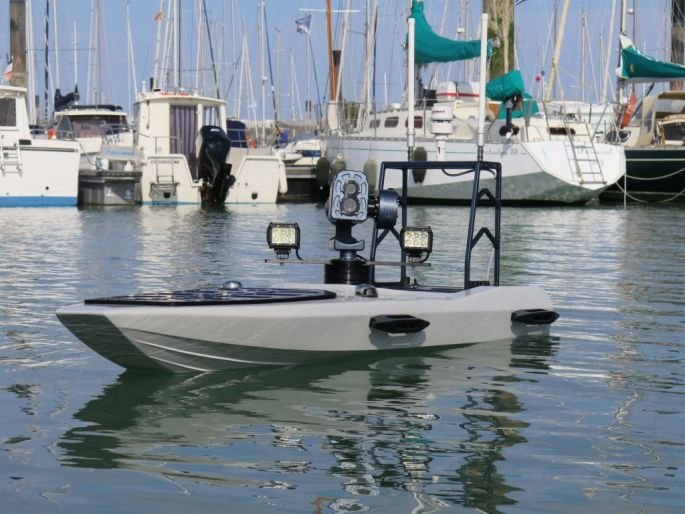
\includegraphics[keepaspectratio=true,height=22mm]{images/bateau_drone.jpg}
\end{center}
\pause
\item Le temps réel n'est pas crucial
\item Plateforme embarquée
\end{enumerate}
\end{block}
\end{frame}

\begin{frame}
\frametitle{Contexte (3)}
De nombreuses approches sont possibles, nous parlerons aujourd'hui d'\textbf{apprentissage profond} et du modèle \textbf{Tiny Yolo} ("You Only Look Once").
\begin{center}
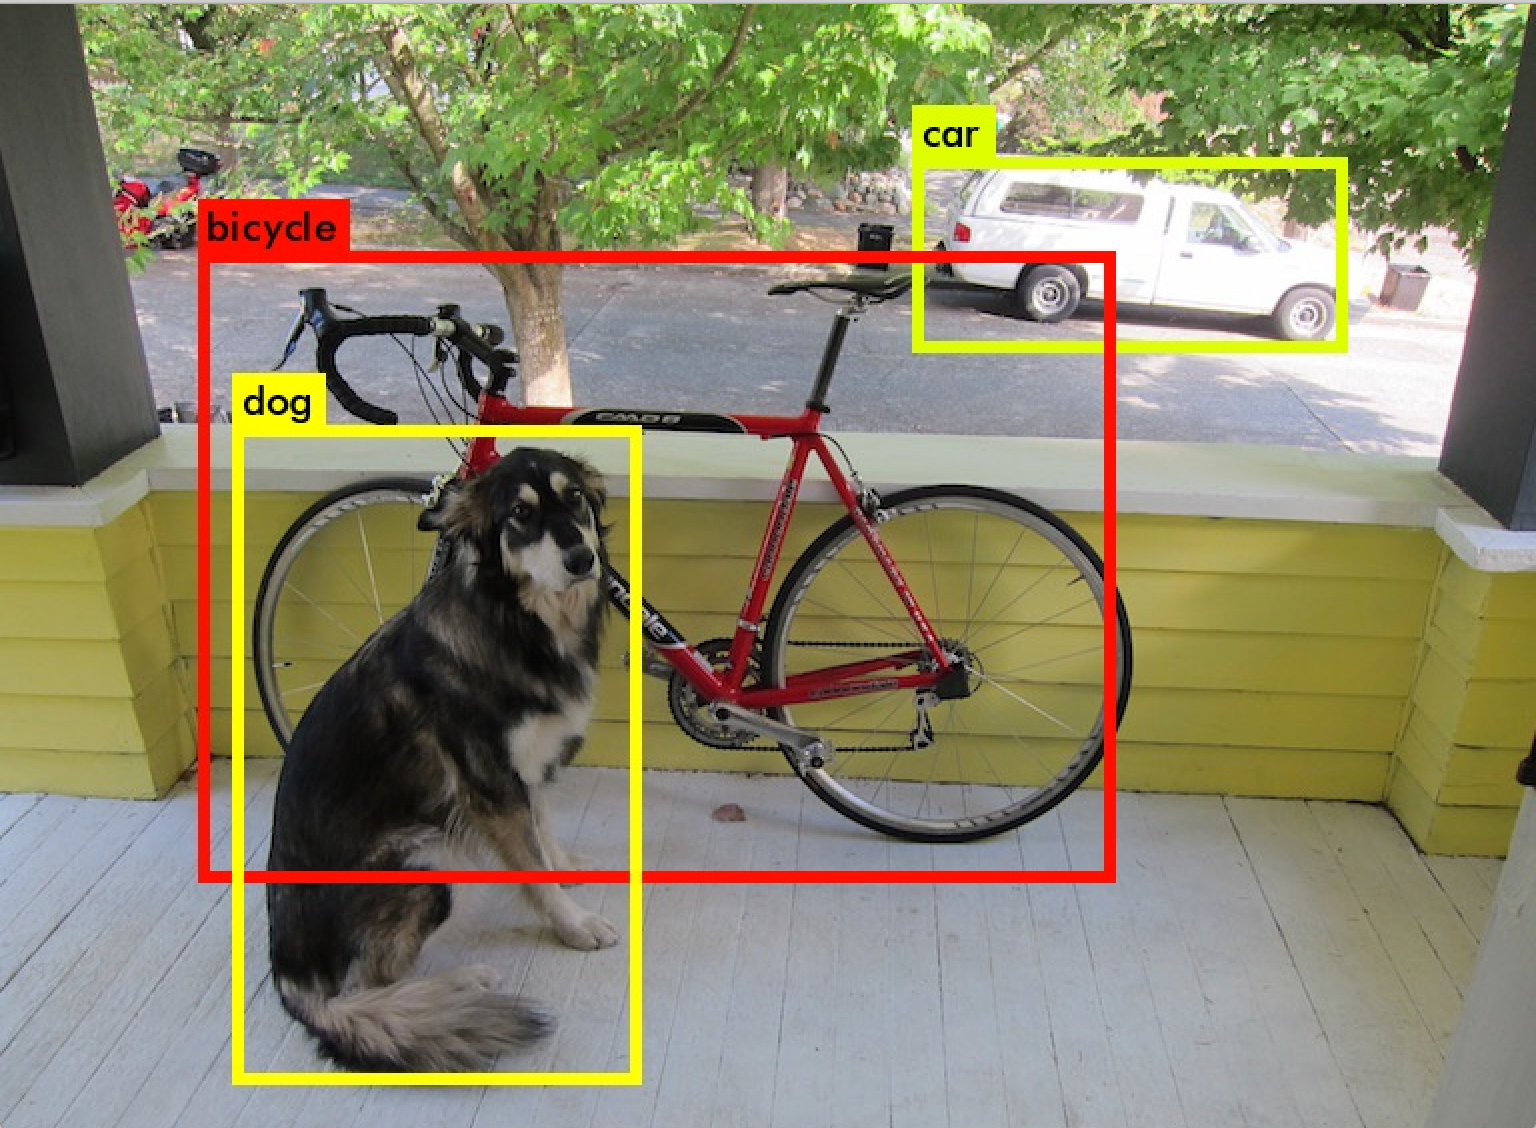
\includegraphics[keepaspectratio=true,width=0.45\textwidth]{images/yolo_works.png}
\hfill
\visible<2>{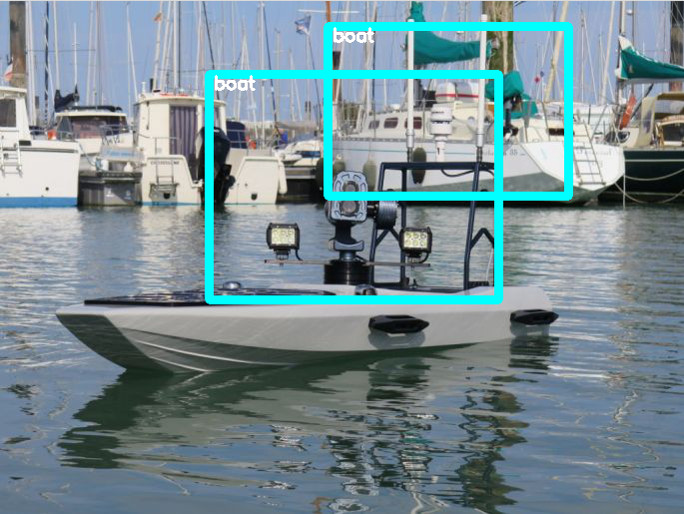
\includegraphics[keepaspectratio=true,width=0.45\textwidth]{images/bateau_drone_predict.jpg}}
\end{center}
\end{frame}

\begin{frame}
\frametitle{Formalisation}
Le modèle Yolo formalise la prédiction d'annotations comme un \textbf{problème de régression} paramétrique:  
 $$f_{\theta} \colon x \mapsto  y$$
\only<1>{\begin{alertblock}{Rappel:}
\begin{center}
\begin{tabular}{cc}
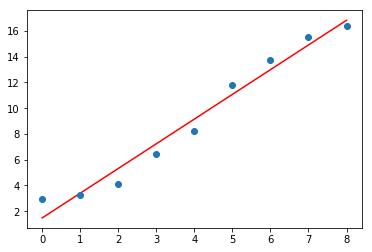
\includegraphics[keepaspectratio=true,width=0.25\textwidth]{images/lin_reg.png} & 
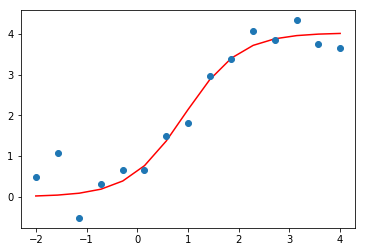
\includegraphics[keepaspectratio=true,width=0.25\textwidth]{images/curve_fit.png}\\
\emph{linregress} & curve\_fit
\end{tabular}
\end{center}
\vspace{-2mm}
Les outils de Scipy sont peu adaptés à l'optimisation séquentielle et aux données massives.
\end{alertblock}}
\only<2>{
Pour Tiny Yolo:
\begin{itemize}
\item la donnée d'entrée $x$ est une image couleur $448 \times 448$
\item la sortie $y$, l'annotation encodée sous la forme d'un vecteur numérique.
\begin{center}

\includegraphics[keepaspectratio=true,width=0.6\textwidth]{images/vecteur_y.pdf}
\end{center}
\end{itemize}
}
\end{frame}

\begin{frame}
\frametitle{Architecture du système : mode prédiction}
Il s'agit de produire une annotation pour une image:
%\vspace{-3mm}
\begin{center}
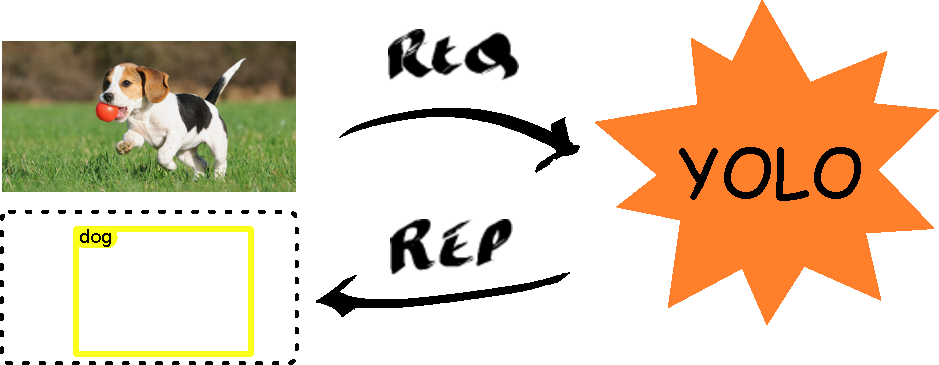
\includegraphics[keepaspectratio=true,height=0.25\textheight]{images/archi_predict.pdf}
\end{center}
%\vspace{-3mm}
\pause
\begin{itemize}
\item Serveur : Tiny Yolo défini en Keras
\pause
\item Client : N'importe quel client qui peut formuler une requête\\ \{ $x$ = image , p\_boxes = [zone à prédire]*\}  au format JSON
\begin{itemize}
\item Bases de données images / Fichiers
\item Interface graphique / Webcam
\item URL / Caméra en ligne
\end{itemize}
\pause
\item Communication entre clients et serveur : Queue \textbf{0-MQ}
\end{itemize}
\end{frame}

\begin{frame}
\frametitle{Serveur: Tiny YOLO}
\vspace{-2mm}
Pourquoi utiliser \textbf{Keras} 
\includegraphics[keepaspectratio=true,height=0.9\baselineskip]{images/keras.png} ?
\begin{itemize}
\item Bibliothèque de haut niveau (TensorFlow, Theano, \emph{etc})
\item Simple, bien documentée, code accessible $\implies$ \textbf{populaire} !
\item Peut être embarquée dans un contexte industriel.
\end{itemize}
\vspace{3mm}
Dans les modèles d'apprentissage profond, le modèle est souvent une \textbf{composition de fonctions} linéaires (convolution, produit matriciel, \emph{etc}) et non linéaires (activation ReLu, SoftMax, \emph{etc}) \textbf{différentiables}.

\begin{center}
%\hfill
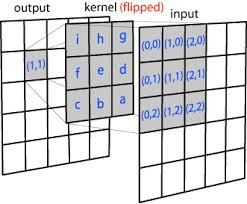
\includegraphics[keepaspectratio=true, width=0.3\textwidth]{images/convolution.jpeg}
\hspace{1cm}
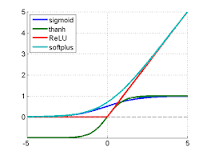
\includegraphics[keepaspectratio=true,width=0.35\textwidth]{images/Relu.png}
%\hfill
%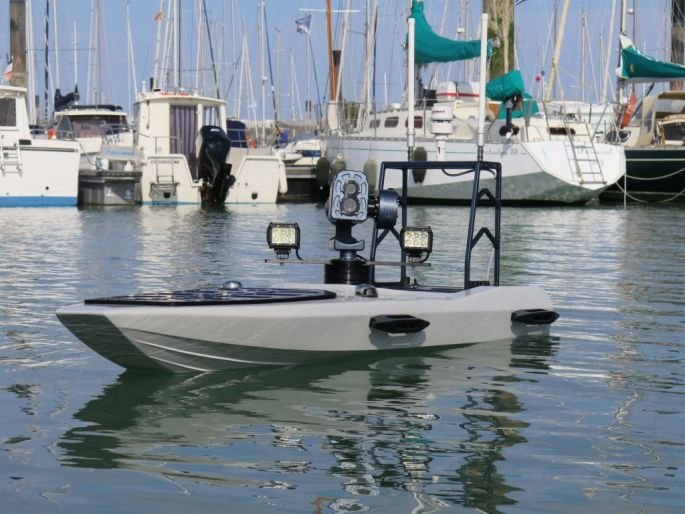
\includegraphics[keepaspectratio=true,width=0.33\textwidth]{images/bateau_drone.jpg}
\end{center}
\end{frame}

\begin{frame}[fragile]
\frametitle{Serveur: Tiny YOLO}
\begin{minipage}[c]{.35\linewidth}
Extrait de code :
\small{
\begin{verbatim}
model = Sequential()
model.add(Conv2D(filters=16, 
       kernel_size=(3, 3), 
       input_shape=(3, 448, 448))
model.add(LeakyReLU(alpha=0.1))
model.add(MaxPooling2D(pool_size=(2,2)))
...
model.add(Dense(1470))

model.load('params.hdf5')
y_pred = model.predict(x)
\end{verbatim}
}
   \end{minipage} 
   \hfill
   \begin{minipage}[r]{.48\linewidth}
   \begin{flushright}
 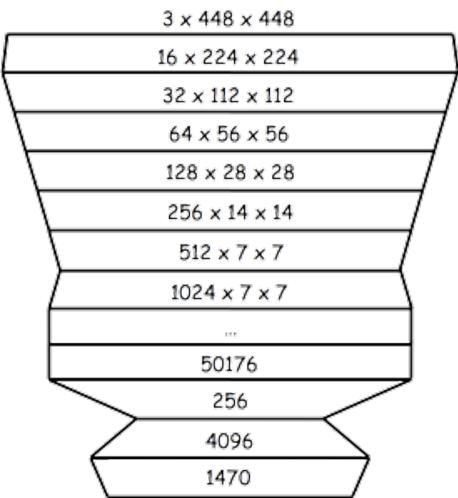
\includegraphics[width=0.73\textwidth]{images/YOLO_params.pdf}
\end{flushright}    
   \end{minipage}
\pause
\begin{alertblock}{En résumé, Tiny Yolo c'est :}
\begin{itemize}
\visible<2->{\item $x: 448 \times 448 \times 3 = 602.112$ prédicteurs}
\visible<3->{\item $y: 1470$ variables à prédire (suivant nombre de classes)}
\visible<4->{\item et $45.089.374$ paramètres !!!}
\end{itemize}
\end{alertblock}
\end{frame}


\begin{frame}
\frametitle{Exemple minimal de client (Prédiction)}
Nous avons choisi le format d'échange JSON:
\begin{center}
\begin{tabularx}{\textwidth}{cc}
\underline{Avantages} & \underline{Inconvénients} \\
\begin{minipage}[l]{.4\linewidth}
\vspace{5mm}
\begin{itemize}
\item Interopérable à l'extérieur de Python
\item Répresentation par une chaîne de caractères
\end{itemize}
\end{minipage}& 
\begin{minipage}[l]{.4\linewidth}
\begin{itemize}
\item Objets simples 
\item Pas de compression
\end{itemize}
\end{minipage}
\end{tabularx}
\end{center}
\pause

Dans le module \textbf{json}, on a seulement besoin de:
\begin{description}
\item[dumps] : encodage
\item[loads] : décodage 
\end{description}
\begin{flushright}
\beamergotobutton{Démo !}
\end{flushright}
\end{frame}



\begin{frame}
\frametitle{Communication Client-Serveur (Prédiction)}
Nous avons choisi la bibliothèque 0-MQ (\textbf{pyzmq})
\begin{itemize}
\item En C++, mais interfacée avec tous les langages.
\item Supporte la communication intra- et inter-machines.
\item Rapide (entrées-sorties asynchrones).
\item Supporte le JSON !
\item Implémente des motifs de communication haut niveau !
\end{itemize}
Nous avons seulement besoin du device Queue:
 \begin{center}
     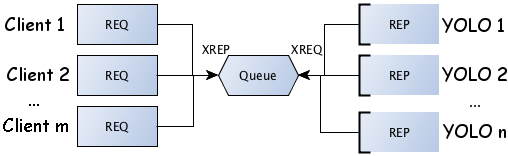
\includegraphics[width=0.7\textwidth]{images/Queue_YOLO.png}
     \end{center}
     \begin{flushright}
\beamergotobutton{Démo !}
\end{flushright}
\end{frame}

\begin{frame}
\frametitle{ Architecture du système : mode entraînement}
%\vspace{-4mm}
On a besoin d'un \textbf{MAXIMUM} d'images annotées:
\vspace{-2mm}
\begin{center}
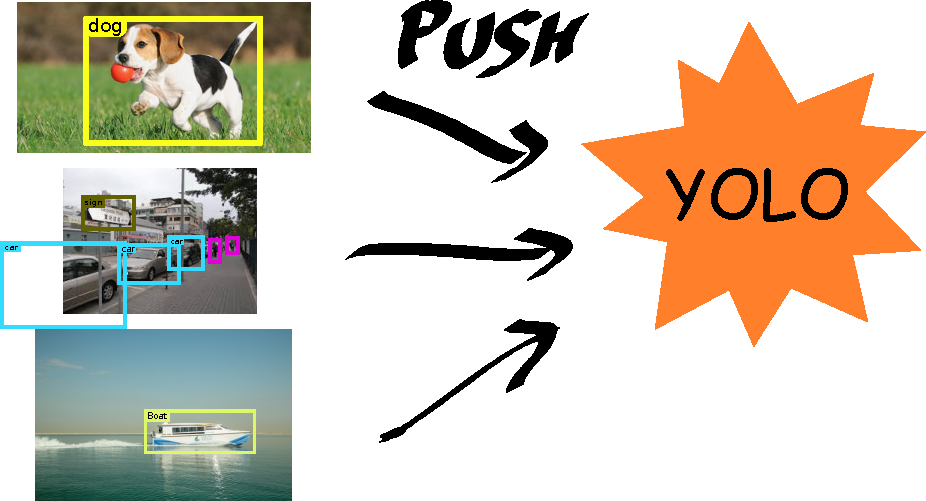
\includegraphics[keepaspectratio=true,height=0.25\textheight]{images/archi_train.pdf}
\end{center}
\pause
\vspace{-3mm}
\begin{itemize}
\item Serveur : Tiny Yolo défini en \textbf{Keras} + 
\includegraphics[keepaspectratio=true,height=2\baselineskip]{images/wizard.png}
\pause
\item Producteurs d'images annotées:
\begin{itemize}
\item Bases d'images (ex: VOC img+xml via \href{https://www.crummy.com/software/BeautifulSoup/}{\textbf{Beautiful Soup}}).
\item Annotations utilisateurs spécifiques à la tâche visée.
\end{itemize}
$$(x = \mbox{image},  \mbox{b\_boxes} = \{(x_1, y_1, x_2, y_2)\}^+, \mbox{labels} = \{0..K\}^+)$$
\end{itemize}
\vspace{-4mm}
\begin{itemize}
\item Communication entre clients et serveur : Streamer \textbf{0-MQ}
\end{itemize}
\end{frame}


\begin{frame}
\frametitle{Communication Prod.-Serv.(Entrainement)}
Nous avons seulement besoin du device Streamer:
\begin{itemize}
\item Communication unidirectionnelle.
\item Protocole JSON.
\item Un seul serveur Yolo.
\end{itemize}
 \begin{center}
     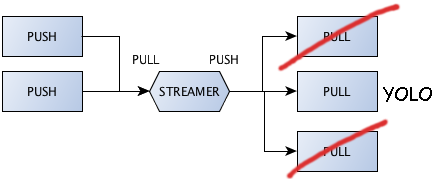
\includegraphics[width=0.7\textwidth]{images/Streamer_YOLO.png}
     \end{center}
\begin{flushright}
\href{http://learning-0mq-with-pyzmq.readthedocs.io/en/latest/pyzmq/devices/streamer.html}{Lien vers l'exemple Streamer \textbf{pyzmq}}
\end{flushright}
\vspace{-2mm}Remarque: \emph{C'est un motif pour la répartition de tâches...}
\end{frame}



\begin{frame}
\frametitle{Serveur: Tiny YOLO (2)}
Quelques tâches du serveur:
\begin{itemize}
\item Encodage de l'annotation JSON vers un vecteur $y$.
\pause
\item Calcul de coût de l'erreur:
\end{itemize}
 \begin{center}
 \invisible<1>{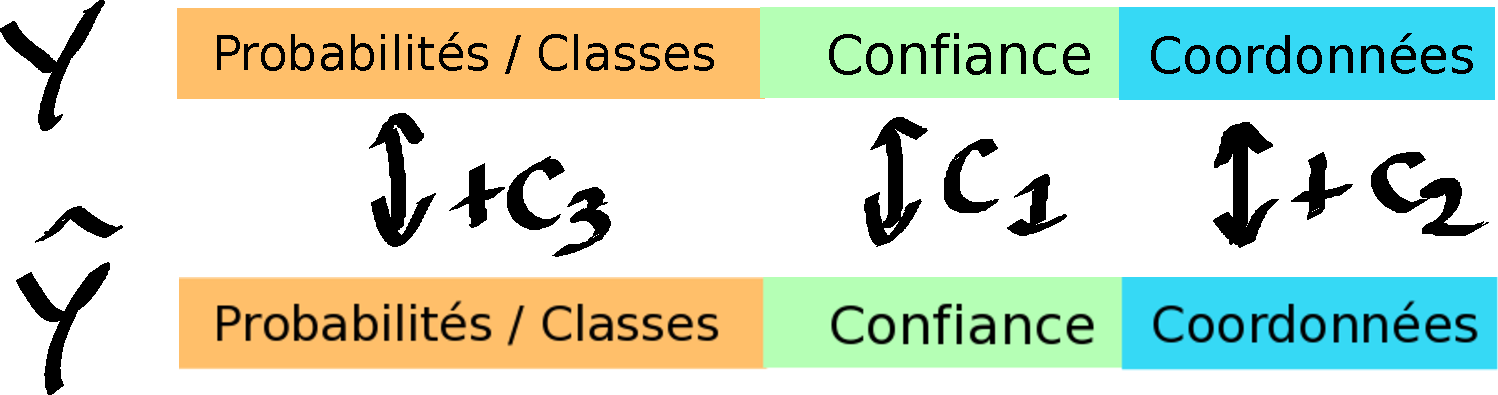
\includegraphics[height=0.22\textheight]{images/loss.pdf}}
 \end{center}
\pause
\begin{itemize}
\item Mettre à jour les 45.089.374 paramètres pour minimiser l'erreur.
\pause
\item Lots, sauvegarde périodique des paramètres, monitoring, \emph{etc}
\end{itemize}
\end{frame}




\begin{frame}
\frametitle{Serveur: Tiny YOLO (2)}
Mais, on va également confier une autre tâche au serveur :
\begin{center}
\shadowbox{Augmenter le nombre d'images annotées !!}\vspace{5mm}
\only<2,4>{
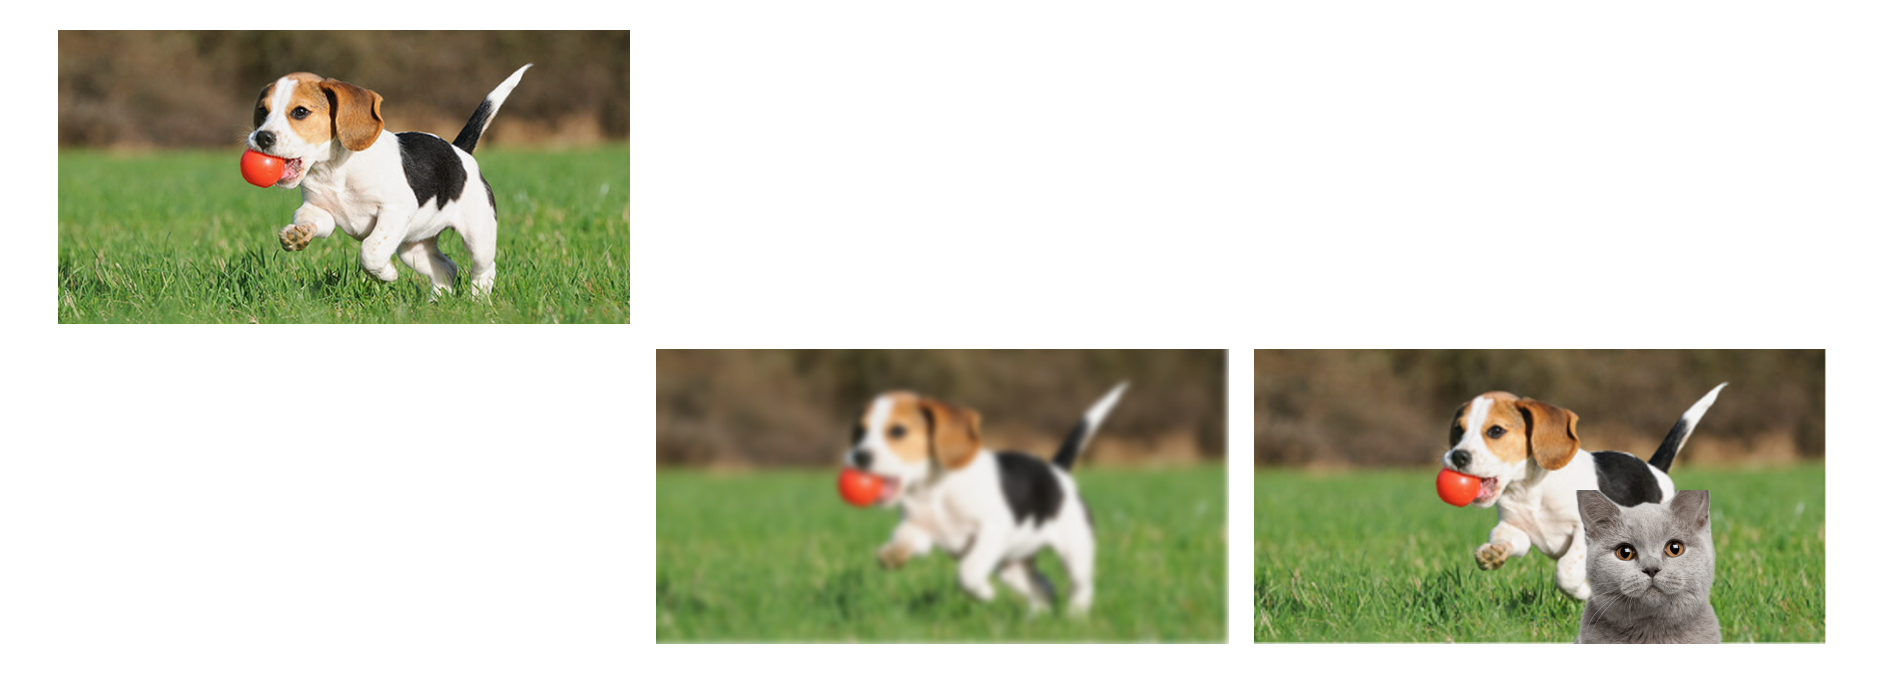
\includegraphics[width=\textwidth]{images/transf_1.png}\\
Plutôt facile à reproduire avec \textbf{OpenCV}
} 
\only<3>{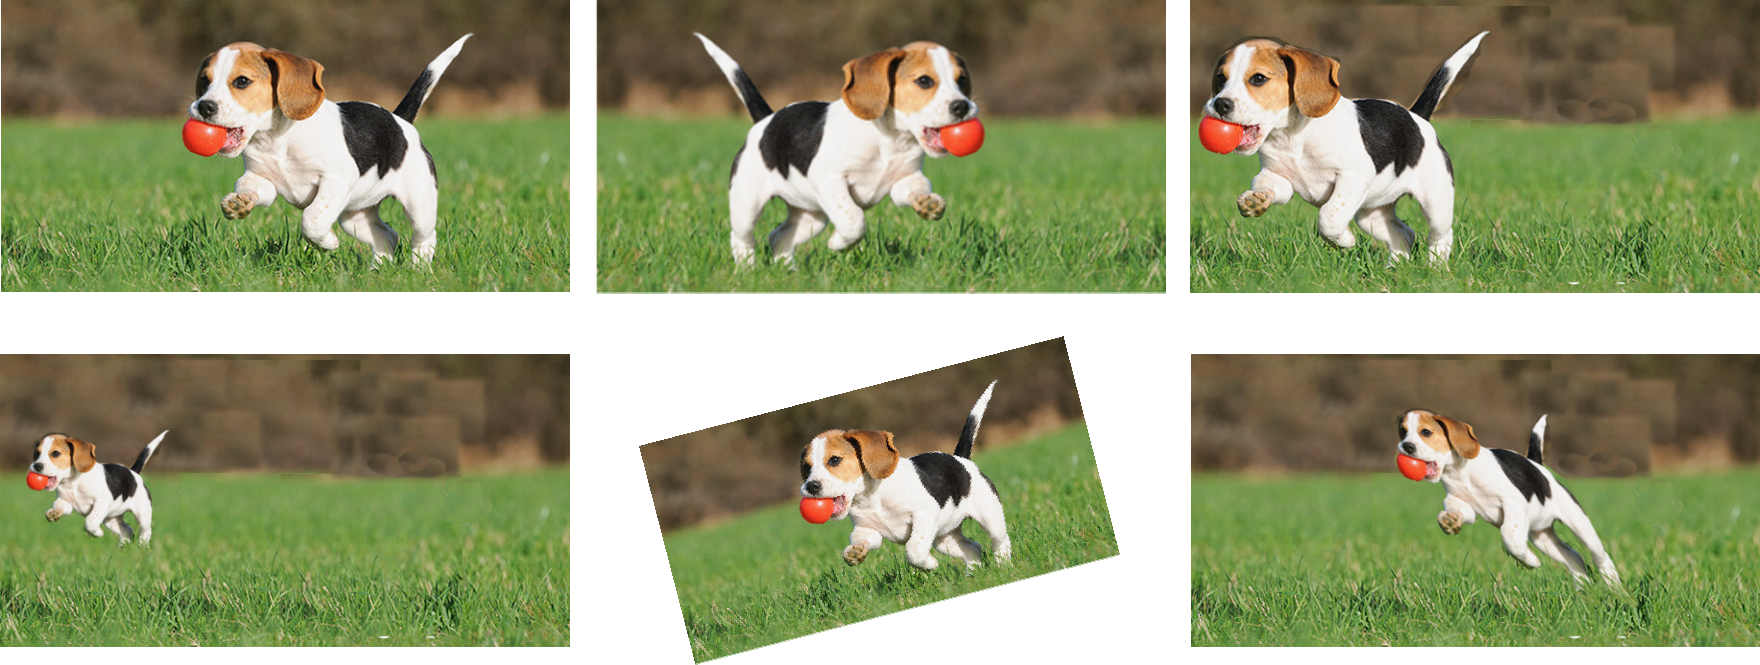
\includegraphics[width=\textwidth]{images/transf_2.pdf}\\
Beaucoup plus compliqué.
} 
\end{center}
\only<4>{\begin{flushright}
\beamergotobutton{Démo !}
\end{flushright}}
\end{frame}

\begin{frame}
\frametitle{Conclusions}
\begin{itemize}
\item Présentation de la méthodologie YOLO pour l'annotation d'images.
\pause
\item Architecture Client/Serveur:
\begin{itemize}
\item Simple : 30 lignes de code, 3 ports ouverts (0-MQ)
\item Puissante : Tout client/fournisseur qui supporte JSON.
\item Adaptable pour d'autres fonctions de serveur \\
(ex. : Collecte de données)
\item Versatile (YOLO est invisible du client)
\end{itemize}
\pause
\item Cadre de développement Recherche:
\begin{itemize}
\item D'autres modèles de régression (architecture, type couches) ...
\item D'autres fonctions de coût ...
\item ... d'autres méthodes d'optimisation.
\item Intégrer des images partielles annotées (ex.: FlickR)
\end{itemize}
\end{itemize}
\end{frame}

\begin{frame}
\frametitle{Perspectives}
\begin{itemize}
\item Finaliser un entraînement de Tiny YOLO des bases existantes.
\item Raffiner les paramètres par rapport au projet.
\item Embarquer le tout dans un prototype (Robot / Drone).
\end{itemize}
\begin{flushright}
\beamergotobutton{Démo !}
\end{flushright}
\end{frame}
\end{document}